\section{METODOLOGI}

% Ubah konten-konten berikut sesuai dengan isi dari metodologi

\subsection{Metode yang digunakan}

Penelitian ini mengikuti metode untuk pengerjaan nya menguki sesuai yang sudah dirancang sebagai berikut

% Contoh input gambar dengan format *.jpg
\begin{figure} [ht] \centering
  % Nama dari file gambar yang diinputkan
  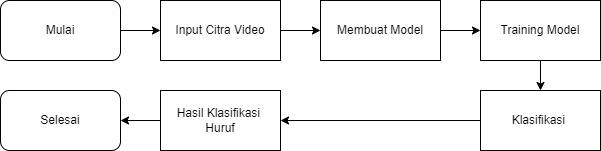
\includegraphics[scale=0.45]{gambar/Metodologi_TA.jpg}
  % Keterangan gambar yang diinputkan
  \caption{\emph{Blueprint} Metodologi Pengerjaan}
  % Label referensi dari gambar yang diinputkan
  \label{fig:Blueprint}
\end{figure}

\subsubsection{Input Citra Video}
Pada tahapan ini , Kamera Webcam akan melakukan deteksi terhadap gestur yang diperagakan . Disini digunakan Library OpenCV dalam rangka untuk membantu menangkap frame yang terdapat di Video 

\subsubsection{Membuat Model}
\begin{figure} [ht] \centering
  % Nama dari file gambar yang diinputkan
  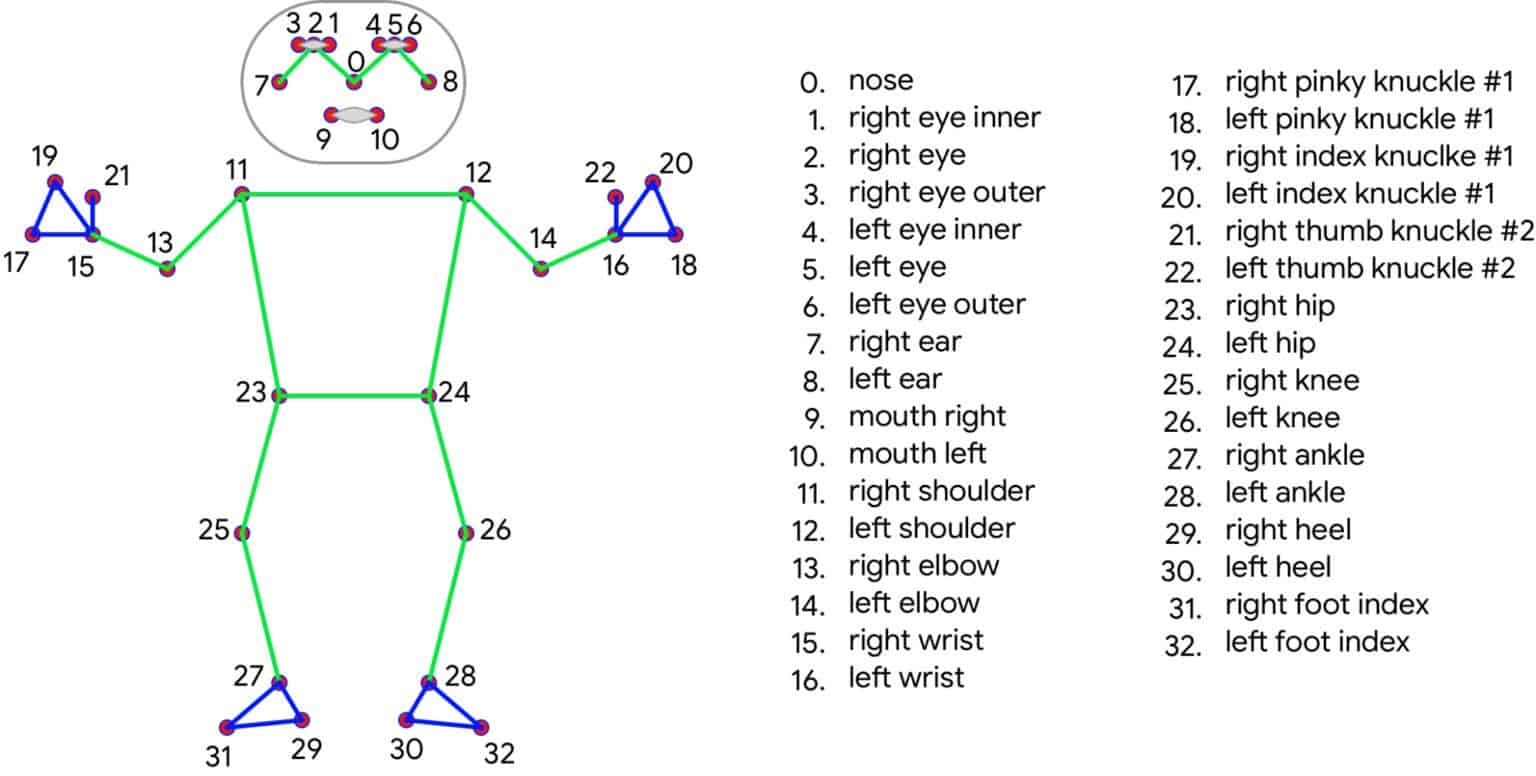
\includegraphics[scale=0.15]{gambar/humanpose.jpg}
  % Keterangan gambar yang diinputkan
  \caption{Model Human Pose dari MediaPipe}
  % Label referensi dari gambar yang diinputkan
  \label{fig:Blueprint}
\end{figure}
Berikutnya dilakukan pembuatan model HumanPose dengan memanfaatkan MediaPipe . Hal ini bertujuan untuk membantu melakukan identifikasi bagian-bagian tubuh manusia dalam citra atau video dalam rangka memperkuat akurasi 

\subsubsection{Training Model}
Selanjutnya dilakukan proses pembelajaran yang digunakan untuk  kemampuan jaringan untuk mengenali dan memprediksi pola dan fitur yang relevan dari input yang diberikan. Training Model menggun

\subsubsection{Klasifikasi}
Setelah dilakukan nya training model sebelumnya menggunakan metode Convolutional Neural Network yang dibantu dengan Estimasi Pose yang dibantu oleh MediaPipe . Klasifikasi ini bertujuan untuk membagi suatu objek ke dalam kelas-kelas tertentu berdasarkan fitur yang dimilikinya

\subsubsection{Hasil Klasifikasi Huruf}
Setelah dilakukan klasifikasi pose semaphore maka didapatkan hasil huruf untuk dikenali
% Contoh penggunaan referensi dari gambar yang diinputkan
% Pada \emph{blueprint} yang tertera di Gambar \ref{fig:Blueprint}. \lipsum[12]

\subsection{Bahan dan peralatan yang digunakan}

\lipsum[13]

\subsection{Urutan pelaksanaan penelitian}

% Ubah tabel berikut sesuai dengan isi dari rencana kerja
\newcommand{\w}{}
\newcommand{\G}{\cellcolor{gray}}
\begin{table}[h!]
  \begin{tabular}{|p{3.5cm}|c|c|c|c|c|c|c|c|c|c|c|c|c|c|c|c|}

    \hline
    \multirow{2}{*}{Kegiatan} & \multicolumn{16}{|c|}{Minggu} \\
    \cline{2-17} &
    1 & 2 & 3 & 4 & 5 & 6 & 7 & 8 & 9 & 10 & 11 & 12 & 13 & 14 & 15 & 16 \\
    \hline

    % Gunakan \G untuk mengisi sel dan \w untuk mengosongkan sel
    Pengambilan data &
    \G & \G & \G & \G & \w & \w & \w & \w & \w & \w & \w & \w & \w & \w & \w & \w \\
    \hline

    Pengolahan data &
    \w & \w & \w & \w & \G & \G & \G & \G & \w & \w & \w & \w & \w & \w & \w & \w \\
    \hline

    Analisa data &
    \w & \w & \w & \w & \w & \w & \w & \w & \G & \G & \G & \G & \w & \w & \w & \w \\
    \hline

    Evaluasi penelitian &
    \w & \w & \w & \w & \w & \w & \w & \w & \w & \w & \w & \w & \G & \G & \G & \G \\
    \hline

  \end{tabular}
\end{table}
